\documentclass[12pt]{article}
\usepackage{graphicx}
\usepackage{appendix}
\usepackage{hyperref}
\usepackage{datatool}
\usepackage{booktabs}
\usepackage{pdflscape}

\title{ Manual for abcngspipelines }

\author{ Alexis Blanchet-Cohen, Bioinformatics analyst \\ alexis.blanchet-cohen@mail.mcgill.ca}
\begin{document}

\maketitle
\thispagestyle{empty} % removes numbering from title page.

\newpage
\tableofcontents
\newpage

\section{Introduction and philosophy}

The intent of abcngspipelines is to provide a flexible and modular framework in which to perform the analysis of next-generation sequencing data.
The pipeline can easily be modified either by changing the parameters in the configuration files, or by editing the source code directly.

The accent is always on simplicity, flexibility and full user control.
One manifestation of this philosophy is that the pipeline never performs the analysis directly. The pipeline simply generates the command scripts. This gives the opportunity to the end-user to verify and manually edit the command scripts.

\section{Configuration files}
There are 3 levels of configuration files: global, project, and user.
The configuration files should follow the INI format.
\[section\]
name=value

\section{Directory structue}
See Figure \ref{figure:directorystructure} for the recommended directory structure for your analyses.
The pipeline is however flexible enough to handle any directory structure.

\begin{figure}[htb]
\centering
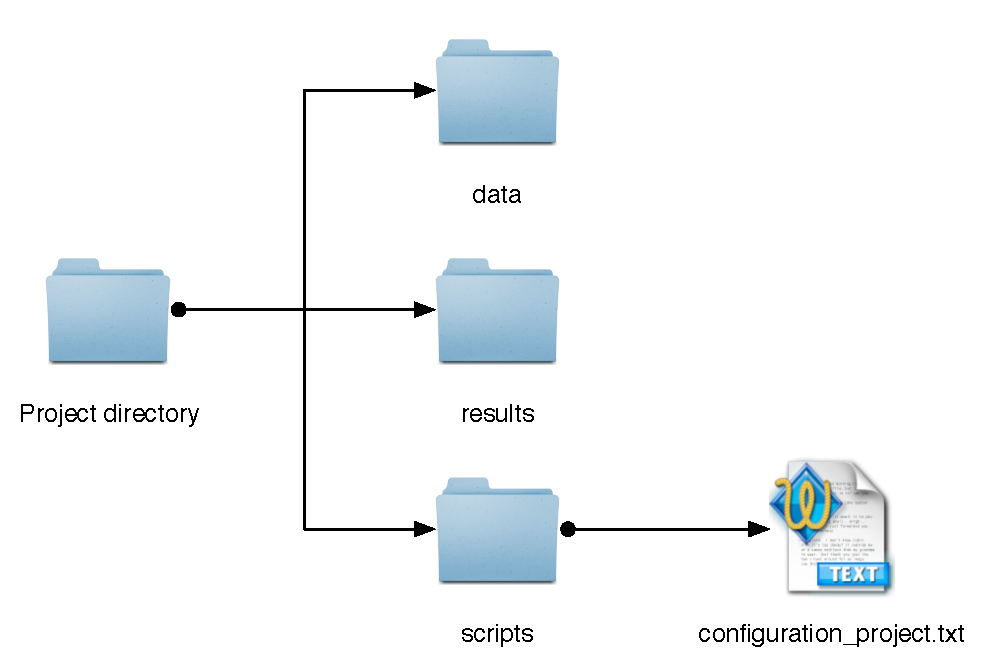
\includegraphics[scale=0.7]{directoryStructure.pdf}
\caption{Directory structure. To make the figure easier to read, a few directories were omitted from this figure.}
\label{figure:directorystructure}
\end{figure}

\section{Requirements}
\begin{itemize}
    \item{Python 3.5+}
    \begin{itemize}
	\item{Pandas module}
    \end{itemize}
\end{itemize}

\section{License}
This software is distributed under the terms of the GNU General Public Licence v3.0.

You are free to use it, and modify it, as long as you give credit to the original authors, and respect the terms of the license.

\clearpage
\bibliography{references}
\bibliographystyle{plain}

\end{document}
                 
